\documentclass{beamer}
\usetheme{Madrid}
\usecolortheme{whale}
%\usepackage{graphicx}
%\graphicspath{{../img/}}
\usepackage[utf8]{inputenc}
\usepackage{graphicx}
\usepackage{hyperref}
\hypersetup{
	colorlinks=true,
	linkcolor=blue,
	filecolor=magenta,      
	urlcolor=cyan,
}	
\usepackage[spanish]{babel}
\usepackage{pdfpages}
\usepackage{booktabs}
\usepackage{color}

\title[Metodología Cuantitativa II]{Introducción a la Regresión Lineal}
\subtitle{Aplicaciónes al estudio de la estructura social}
\author{German Rosati \\  \href{ german.rosati@gmail.com}{german.rosati@gmail.com}}
\institute{UNTREF - UNSAM - CONICET}
\date{\today}
%\logo{\includegraphics[height=0.4cm]{img/header-logo.png}}

\begin{document}
\frame{\titlepage}
%\begin{frame}
%	\frametitle{Hoja de ruta}
%	\tableofcontents
%\end{frame}

\begin{frame}
\frametitle{Hoja de ruta}
\framesubtitle{Temas a tocar}
\textbf{Modelos de regresión lineal y logística}
	\begin{itemize}
		\item Forma funcional
		\item Interpretación de parámetros
		\item Evaluación
		\item Problemas...
	\end{itemize}	
\end{frame}

\section{Repaso...}
\begin{frame}
\frametitle{Repaso... }
\framesubtitle{¿Qué es un modelo?}
	\begin{itemize}
		\item Forma de proponer hipótesis sobre la forma en que se combinan variables
		\item En general, tienen esta forma 
			\begin{equation}
				Y = f(X) + \epsilon
			\end{equation}
		\item Problema: estimar $f(X)$
		\begin{itemize}
			\item Suponer que $Y$ es una combinación lineal de las $X$ 
			\item A su vez $Y$ es una variable cuantitativa
			\item Terreno propicio para la \textbf{regresión lineal}
		\end{itemize}
	\end{itemize}
\end{frame}


\section{Regresión Lineal}
\subsection{Fundamentos}
\begin{frame}
	\frametitle{Regresión Lineal Múltiple}
	\framesubtitle{Fundamentos}
	\begin{itemize}
		\item{En una regresión lineal, asumimos que la relación entre los predictores $X$ y la respuesta $Y$ toma la siguiente forma}
		\begin{equation}
			y_{i} = \beta_{0} + \beta_{1}X_{1} + \beta_{2}X_{2} +...+ \beta_{p}X_{p} + \epsilon
		\end{equation}
		
		\item{En general, buscaremos estimar los parámetros del modelo, por lo cual, dadas las estimaciones $\hat{\beta}_{0}$ y $\hat{\beta}_{j}$, definimos una nueva predicción del valor $\hat{Y}$ como}
		
		\begin{equation}
		\hat{y_{i}} = \hat{\beta_{0}} + \hat{\beta_{1}}X_{1} + \hat{\beta_{2}}X_{2} +...+ \hat{\beta_{p}}X_{p} + \epsilon
		\end{equation}
		
		\item{$\beta_{0}$ es el intercepto y $\beta_{j}$ es la pendiente para la variable $X_{j}$}
		\end{itemize}
\end{frame}

\begin{frame}
	\frametitle{Regresión Lineal}
	\framesubtitle{Fundamentos}
	\begin{itemize}
		\item{Si $\hat{y_{i}}$ representa la predicción para el i-ésimo caso condicionado a los valores de $X_{i}$, $\implies$ $\epsilon_{i} = (\hat{y_{i}} - y_{i})$ es el \emph{residuo} para ese i-ésimo caso}
		\item{Definimos a la suma de los residuos al cuadrado (RSS) como $RSS = \epsilon_{1}^2 + \epsilon_{2}^2 + \epsilon_{3}^2 + ... + \epsilon_{n}^2$. o, de forma equivalente}
	
		\item{Buscamos estimar los valores de $\beta_{0}, \beta_{1}, ..., \beta_{p}$ como el valor que minimiza el RSS}	
		
		\begin{equation}
			\begin{aligned}
			RSS & = \sum_{i=1}^{n}(y_{i} - \hat{y_{i}})^2 \\
		    & =  \sum_{i=1}^{n}(y_{i} - \hat{\beta_{0}} - \hat{\beta_{1}}X_{1} - \hat{\beta_{2}}X_{2} - ... - \hat{\beta_{p}}X_{p})^2 
			\end{aligned}
		\end{equation}
		\item{$RSS$ es una medida de la variabilidad de la variable dependiente que NO es explicada por nuestro modelo... nuestra ``ignorancia''}
	\end{itemize}
\end{frame}

\begin{frame}
\frametitle{Regresión Lineal}
\framesubtitle{Ejemplo 1}
\begin{itemize}
	\item Modelo simple: predecir las ventas de una emprsa en función del gasto que realizan en publicidad para TV
	\item ¿Cuántas variables hay?
	\item ¿Qué función cumple cada una?

	\begin{equation}
	\begin{aligned}
    	Y & =      \beta_{0} + \beta_{1}X + \epsilon \\
		sales & =  \beta_{0} + \beta_{1} x TV + \epsilon
	\end{aligned}
	\end{equation}
	\item Asumimos que la relación es \textit{lineal}
\end{itemize}
\end{frame}


\begin{frame}
\frametitle{Regresión Lineal}
\framesubtitle{Ejemplo 1}
\begin{columns}
	\begin{column}{0.35\textwidth}
	\begin{itemize}
		\item Infinitas rectas pasan por esta nube de puntos
		\item Cada una se caracteriza por un set de parámetros: $(\beta_{0}, \beta_{1})$
		\item Queremos encontrar la que mejor ajusta: la que minimiza el $RSS$
	\end{itemize}
	\end{column}
	\begin{column}{0.58\textwidth}
		\centering
		\begin{figure}[h]	
			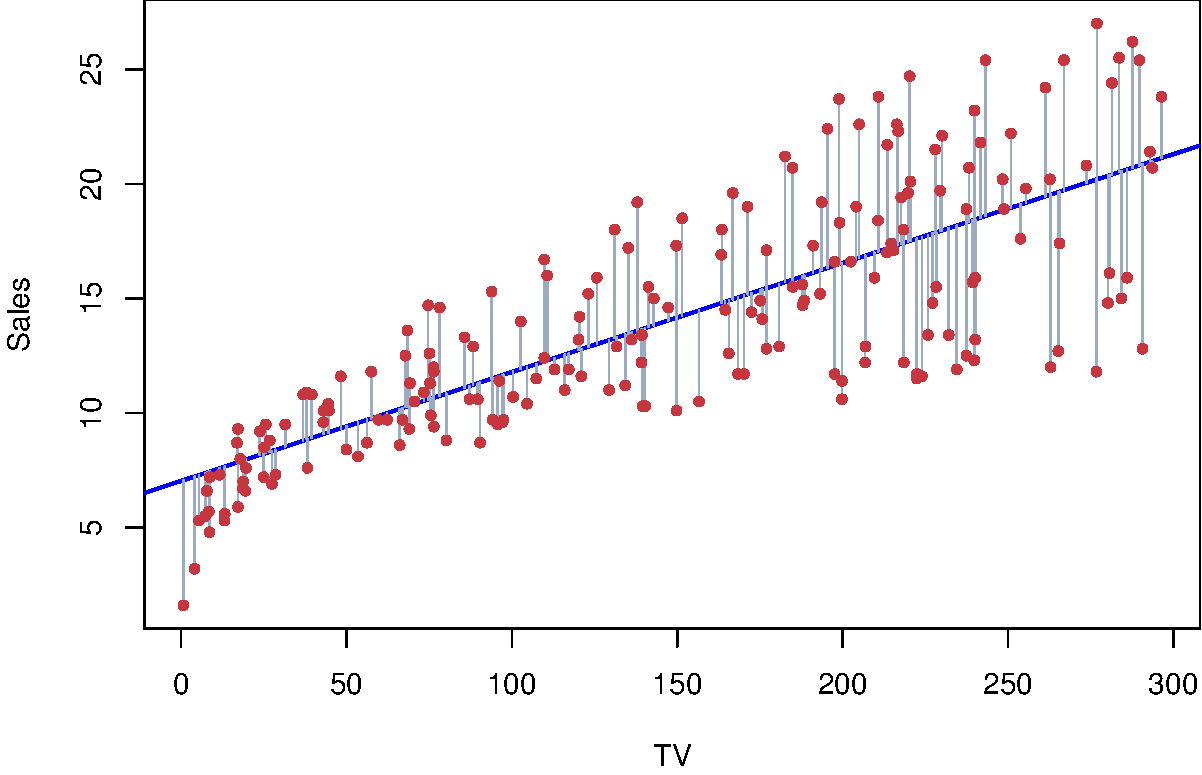
\includegraphics[width=0.95\linewidth, height=0.6\textheight]{./img/pdf/3_1}
			\caption{Scatter plot de gasto en TV y ventas \cite{hastie02}}
		\end{figure}
	\end{column}
\end{columns}
\end{frame}

\begin{frame}
\frametitle{Regresión Lineal}
\framesubtitle{Ejemplo 1}
\begin{columns}
	\begin{column}{0.5\textwidth}
		\centering
		\begin{figure}[h]
			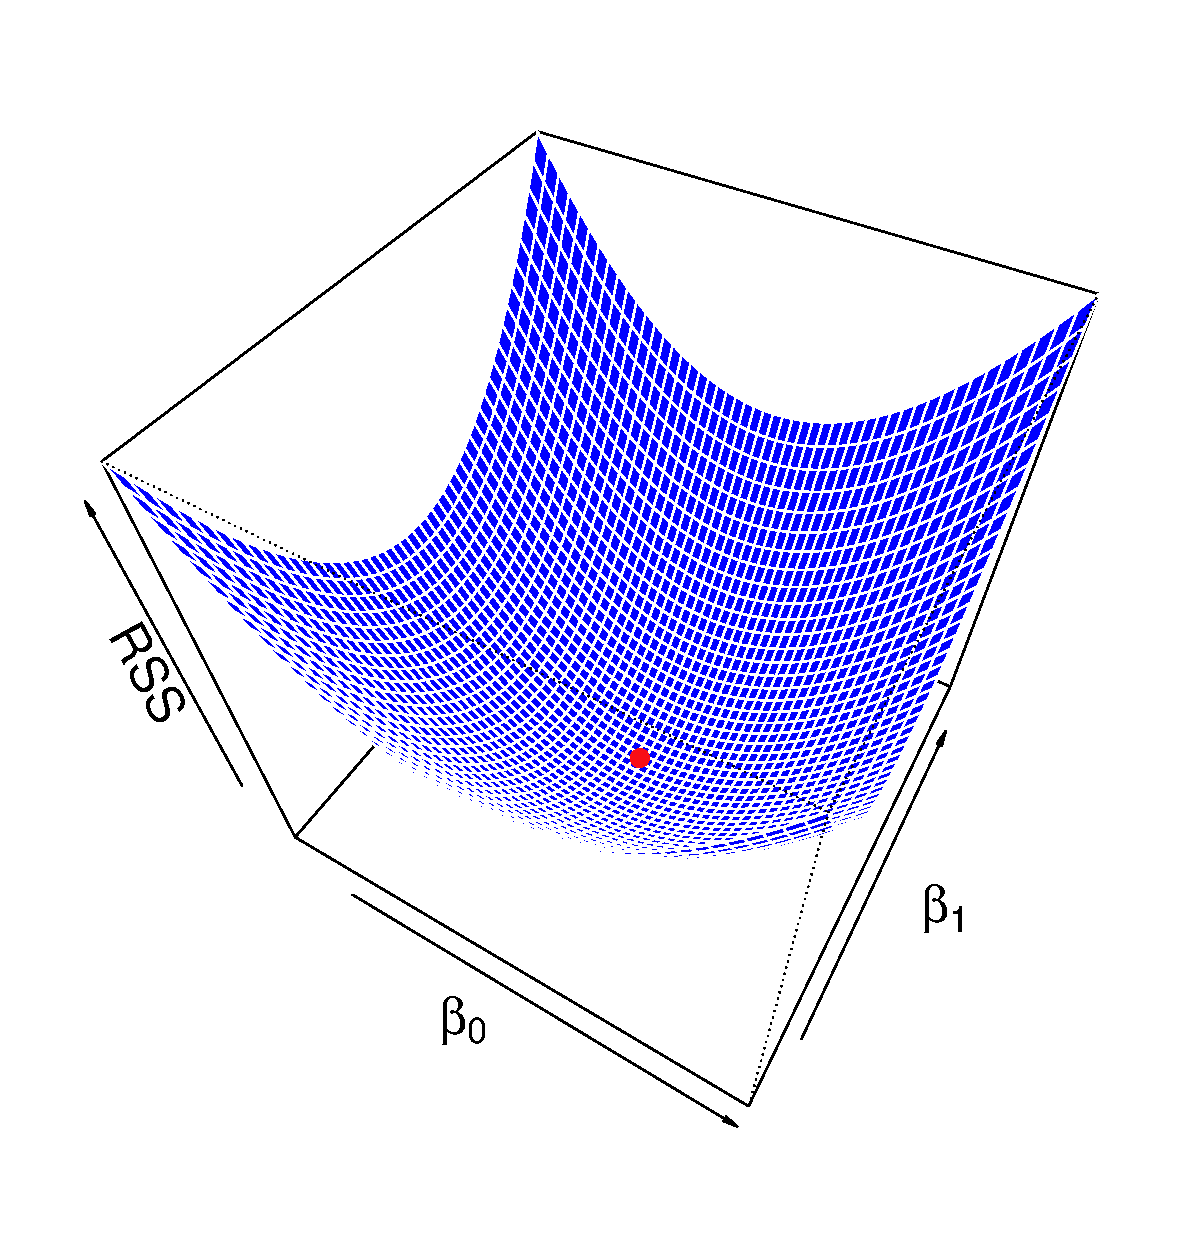
\includegraphics[width=0.95\linewidth, height=0.6\textheight]{./img/pdf/3_2b}
			\caption{Esquema de valores de $RSS$ en función de $\beta_{0}$ y $\beta_{1}$ \cite{hastie02}}
		\end{figure}
	\end{column}
	\begin{column}{0.35\textwidth}
		\begin{itemize}
			\item Para cada combinación $(\beta_{0}, \beta_{1})$ se podría calcular su $RSS$ correspondiente.
			\item Intuición: pruebo todas las combinaciones posibles de $(\beta_{0}, \beta_{1})$ y elijo la de menor $RSS$
		\end{itemize}
	\end{column}
\end{columns}
\end{frame}


\begin{frame}
\frametitle{Regresión Lineal}
\framesubtitle{Ejemplo 1}
\begin{columns}
	\begin{column}{0.5\textwidth}
		\centering
		\begin{figure}[h]
		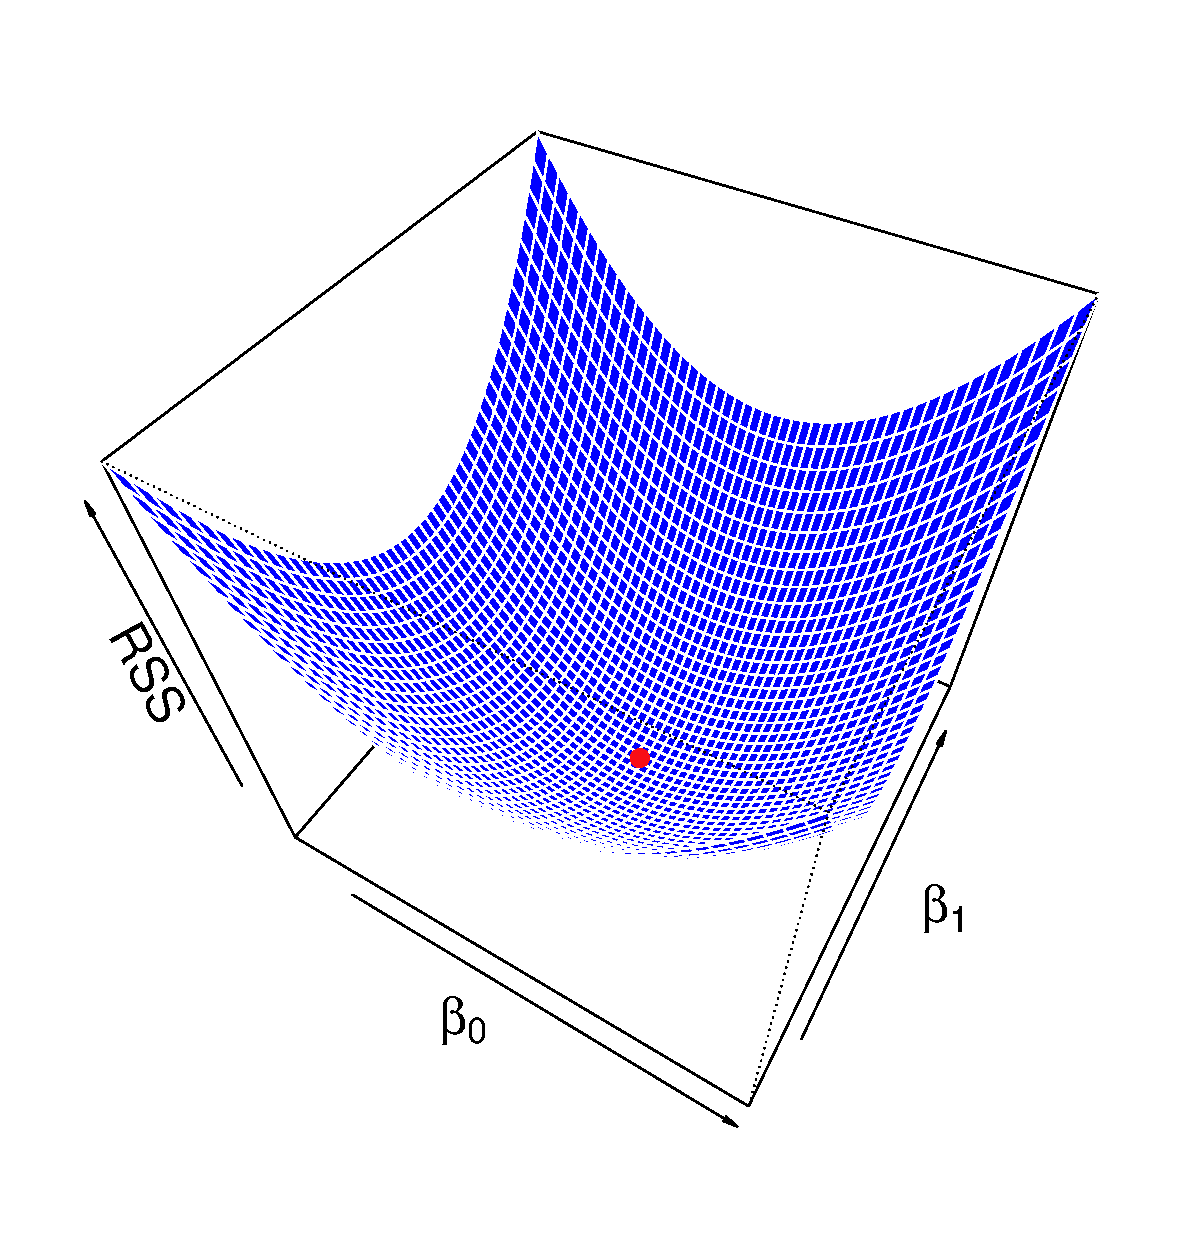
\includegraphics[width=0.95\linewidth, height=0.6\textheight]{./img/pdf/3_2b}
		\caption{Esquema de valores de $RSS$ en función de $\beta_{0}$ y $\beta_{1}$ \cite{hastie02}}
		\end{figure}
	\end{column}
	\begin{column}{0.5\textwidth}
		\begin{itemize}
			\item En regresión lineal forma analítica de resolucion. Derivando sobre la ecuación del $RSS$ se obtienen las ecuaciones normales:
					
			\begin{equation}
				\begin{aligned}
					\beta_{1} & = \frac{\sum (X_{i} - \bar{X})(Y_{i} - \bar{Y})}{\sum(X_{i} - \bar{X})^2} \\
					\beta_{0} & = \bar{y} - \beta_{1}\bar{X} 
				\end{aligned}
			\end{equation}
			
			\item Otros métodos... Descenso de gradiente
		\end{itemize}
	\end{column}
	
\end{columns}
\end{frame}


\begin{frame}
\frametitle{Regresión Lineal}
\framesubtitle{Ejemplo 1 - Coeficientes}
	\begin{figure}[h]
		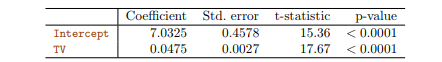
\includegraphics[width=1.\linewidth, height=0.2\textheight]{./img/table01}
		\caption{Coeficientes $\beta$ estimados para TV y Sales \cite{hastie02}}
		\end{figure}
	\begin{itemize}
		\item ¿Cómo se interpretan?: $\beta_{p}$ Efecto marginal
		\item ¿Qué significa cada columna de la tabla?
	\end{itemize}	
\end{frame}

\begin{frame}
\frametitle{Regresión Lineal}
\framesubtitle{Ejemplo 1 - Coeficientes}
Intervalo de confianza
	\begin{itemize}
		\item Error estándard:
			 \begin{flalign}
				 SE(\beta_{1})^2 &= \frac{\sigma^2}{\sum_{i=1}^n(x_{i}-\bar{x})^2} 
			 \end{flalign}
		\item Intervalo de confianza:
			\begin{equation}
				\large \beta_{1} \pm 2 \times SE(\beta_{1})
			\end{equation}
		\item Hay un aproximadamente un 95\% de chances de que el intervalo contenga el valor verdadero del parámetro.
		\item Para el ejemplo, el intervalo de confianza de 95\% para $\beta_{1}$ es $[0.042, 0.053]$
	\end{itemize}	
\end{frame}

\begin{frame}
\frametitle{Regresión Lineal}
\framesubtitle{Ejemplo 1 - Coeficientes}
Test de hipótesis
\begin{itemize}
	\item Hipótesis más común:
	\begin{itemize}
		\item $H_{O}:$ No hay relación entre $X$ y $Y$ | $\beta_{1} = 0$ 
		\item $H_{A}:$ Hay relación entre $X$ y $Y$ | $\beta_{1} \neq 0$
	\end{itemize}
	\item Estadístico t:
		\begin{equation}
			t = \frac{\beta_{1} - 0}{SE(\beta_{1})}
		\end{equation}
\end{itemize}	
\end{frame}


\begin{frame}
\frametitle{Regresión Lineal}
\framesubtitle{Ejemplo 1 - Ajuste}

Muchas medidas:
\linebreak
	\begin{itemize}
		\item Coeficiente de determinación:
			\begin{equation}
				R^2 = \frac{TSS-RSS}{TSS} = 1-\frac{RSS}{TSS}
			\end{equation} \\
			dónde $TSS=\sum_{i=1}^n(y_{i}-\bar{y})^2$ \\

			Es decir, la proporción de la varianza de la variable dependiente que es explicada por el modelo
		\item{$MSE=\frac{1}{n}\sum_{i=1}^n(y_{i}-\hat{y_{i}})^2$}
		\item{$RMSE=\sqrt{\frac{1}{n}\sum_{i=1}^n(y_{i}-\hat{y_{i}})^2}$}
		
	\end{itemize}
\end{frame}

\section{Regresión Lineal Múltiple}
\begin{frame}
\frametitle{Regresión Lineal Múltiple}
\framesubtitle{Volvamos al comienzo...}

	\begin{equation}
		y_{i} = \beta_{0} + \beta_{1}X_{1} + \beta_{2}X_{2} +...+ \beta_{p}X_{p} + \epsilon
	\end{equation}

\begin{itemize}
	\item Interpretamos cada $\beta_{j}$ como el efecto promedio sobre $Y$ \textit{mantiendo todos los demás factores -$X's$- constantes}
	\item Nuestro modelo se transforma en
		 \begin{equation}
		 sales  =  \beta_{0} + \beta_{1} \times TV + \beta_{2} \times radio + \beta_{3} \times diarios + \epsilon	 	
\end{equation}
	\end{itemize}
\end{frame}

\begin{frame}
\frametitle{Regresión Lineal Múltiple}
\framesubtitle{Interpretación}
\begin{itemize}
	\item{\emph{Escenario ideal:}}
	\begin{itemize}
		\item{Diseño balanceado}
		\item{Cada coeficiente puede ser interpretado y testeado de forma separada}
		\item{Las interpretaciones estilo ``efecto de $X_{j}$ sobre $Y$ manteniendo el resto constante'' son viables}
	\end{itemize}
	\item{La correlación entre los predictores trae problemas}
	\begin{itemize}
		\item{La varianza de los predictores tiende a aumentar}
		\item{Las interpretaciones se vuelven más imprecisas: no funciona el ``manteniendo todo lo demás constante'' porque cuando $X_{j}$ cambia, el resto también}	
	\end{itemize}
	\item{Abstenerse de hacer interpretaciones causales}
\end{itemize}
\end{frame}


\begin{frame}
\frametitle{Regresión Lineal Múltiple}
\framesubtitle{Ejemplo 2}
\begin{figure}[h]
	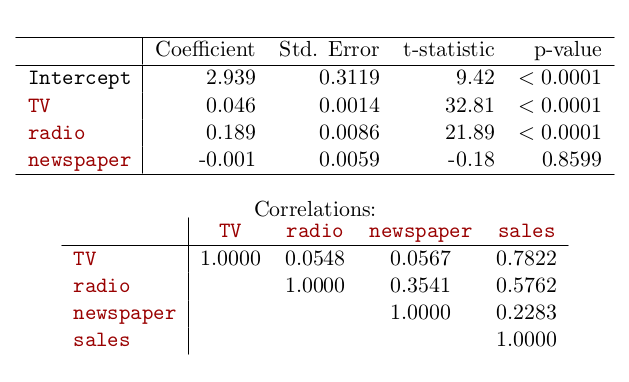
\includegraphics[width=0.8\linewidth, height=0.6\textheight]{./img/table02}
	\caption{Coeficientes $\beta$ estimados para TV, radio, diarios y Sales \cite{hastie02}}
\end{figure}
\end{frame}

\begin{frame}
	\frametitle{Regresión Lineal Múltiple}
	\framesubtitle{Algunas preguntas relevantes}
	\begin{itemize}
		\item¿Es al menos uno de los predictores relevantes para la predicción de $y$?
		\begin{itemize}
			\item Estadístico F:
			
			\begin{equation}
				F = \frac{(TSS - RSS) / p}{RSS/(n-p-1)}
			\end{equation}
		
		\end{itemize}

\begin{figure}[h]
	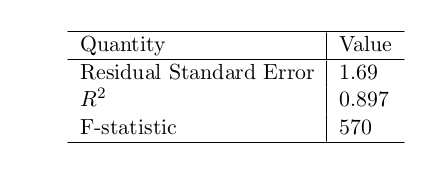
\includegraphics[width=0.5\linewidth, height=0.25\textheight]{./img/table03}
	\caption{Prueba $F$ y $R^2$ para regresión completa \cite{hastie02}}
\end{figure}
		
		
		%\item{¿Cuál (o cuáles) de las variables independientes ayudan a explicar $y$?}
		%\item{¿Cuál es el ajuste del modelo? ¿Cómo medirlo?}
	\end{itemize}
\end{frame}



\begin{frame}
	\frametitle{Regresión Lineal Múltiple}
	\framesubtitle{Evaluación: ¿Qué variables son importantes?}
	\begin{itemize}
		\item{Área más amplia llamada \emph{model selection}}
		\item{Muchos enfoques y técnicas}
		\begin{itemize}
			\item{\textbf{Best Subset Selection:} ajustamos todos los modelos posibles para todos los subsets de variables y elegimos el mejor basado en alguna métrica de error. \\
			\emph{Problema:} generalmente no podemos examinar TODOS los modelos posibles. Hay $2^p$ modelos posibles. Para $p=40$ hay más de 1.000.000.000 de modelos.\\
			Necesitamos algún enfoque de selección automático y que achique el espacio de búsqueda}
		\end{itemize}
	\end{itemize}
\end{frame}

\begin{frame}
	\frametitle{Regresión Lineal Múltiple}
	\framesubtitle{Evaluación: ¿Qué variables son importantes?}
	\begin{itemize}
		\item{\textbf{Forward Selection:}}
		\begin{enumerate}
			\item{Empezamos con modelo nulo: contiene solo $\beta_{0}$}
			\item{Fiteamos $p$ modelos simples (un predictor) y elegimos el mejor en térmimos de $RSS$}
			\item{Agregamos a ese modelo la variable que mejor funciona en un modelo de dos variables}
			\item{Seguimos hasta que se cumple algún criterio de corte}
		\end{enumerate}
	\end{itemize}
\end{frame}

\begin{frame}
	\frametitle{Regresión Lineal Múltiple}
	\framesubtitle{Evaluación: ¿Qué variables son importantes?}
	\begin{itemize}
		\item{\textbf{Backward Selection:}}
		\begin{enumerate}
			\item{Empezamos con un modelo con todas las variables}
			\item{Eliminamos la variable con mayor p-valor en la prueba t}
			\item{Fiteamos el nuevo modelo con $(p-1)$ variables y volvemos a eliminar la variable con mayor p-valor}
			\item{Seguimos hasta que se cumple algún criterio de corte}
		\end{enumerate}
	\end{itemize}
\end{frame}

\begin{frame}
	\frametitle{Regresión Lineal Múltiple}
	\framesubtitle{Evaluación: ¿Qué variables son importantes?}
	\begin{itemize}
		\item{Hay muchos criterios para elegir un modelo ``óptimo'' en el camino de modelos construidos por la selección Forward o Backward}
		\begin{itemize}
			\item{\emph{Cp de Mallow}}
			\item{\emph{Akaike Information Criteria} (AIC)}
			\item{\emph{Bayesian Information Criteria} (BIC)}
			\item{\emph{$R^2$ ajustado}}
			\item{\emph{Cross-Validation}}
		\end{itemize}
	\end{itemize}
\end{frame}

\subsection{Extensiones del Modelo lineal}
\begin{frame}
\frametitle{Extensiones de Modelo Lineal}
\framesubtitle{Interacciones entre predictores}
	\begin{itemize}
		\item{Pese a su simplicidad, es posible agregar complejidad a un modelo lineal}
		\item{Podemos modelar la interacción entre predictores a través del producto $X_{1}X_{2}$}
		\item{El modelo adquiere la siguiente forma}
		\begin{equation}
			\begin{aligned}
				y_{i} & = \beta_{0} + \beta_{1}X_{1} + \beta_{2}X_{2} + + \beta_{3}X_{1}X_{2} + \epsilon \\
				& =  \beta_{0} + (\beta_{1} + \beta_{3} X_{2}) X_{1} + \beta_{2}X_{2} + \epsilon 
			\end{aligned}
		\end{equation}
		\item{\emph{Principio jerárquico:} si se incluye una interacción en el modelo, debe incluirse también los efectos de orden menor (aún cuando los p-valores no sean significativos)}	
	\end{itemize}
\end{frame}

\begin{frame}
\frametitle{Extensiones del Regresión Lineal}
\framesubtitle{Interacciones entre predictores - Ejemplo 3}
\begin{itemize}
	\item Supongamos que en el modelo anterior que el impacto de un incremento del gasto en TV afecta de alguna forma la efectividad de gasto en radio
	\item En esta situación, dado un presupuesto fijo quizás sea más efectivo alocarlo en ambas variables
	\item Efecto interacción
\end{itemize}
\end{frame}


\begin{frame}
\frametitle{Extensiones del Regresión Lineal}
\framesubtitle{Interacciones entre predictores - Ejemplo 3}
\begin{itemize}
	\item Nuestro modelo:
	\begin{equation}
	\begin{aligned}
	sales & = \beta_{0} + \beta_{1} \times TV + \beta_{2} \times radio + + \beta_{3} \times radio \times TV + \epsilon \\
	& =  \beta_{0} + (\beta_{1} + \beta_{3} \times  radio) \times  TV + \beta_{2}\times radio + \epsilon
	\end{aligned}
	\end{equation}
	\item Resultados
	
	\begin{figure}[h]
		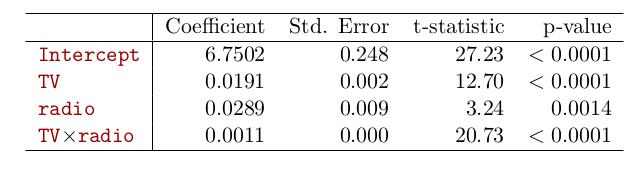
\includegraphics[width=0.7\linewidth, height=0.25\textheight]{./img/table04}
		\caption{Resultados de regresión con términos de interacción\cite{hastie02}}
	\end{figure}
	
	\end{itemize}
\end{frame}


\begin{frame}
\frametitle{Extensiones del Regresión Lineal}
\framesubtitle{Interacciones entre predictores - Ejemplo 3}
\begin{itemize}
	\item ¿Es relevante la interacción?
	\item $R^2 = 0.98$ ¿Qué pueden decir del ajuste respecto al modelo anterior?
	\item Los coeficientes sugieren que un incremento de la publicidad en TV de \$1.000 se asocia con un incremento en las ventas de ($\beta_{1} + \beta_{3} \times radio) \times 1.000 = 19 + 1.1 \times radio$
\end{itemize}
\end{frame}

\begin{frame}
	\frametitle{Extensiones del Modelo Lineal}
	\framesubtitle{Introduciendo no linealidad}
	\begin{itemize}
		\item{Diferentes formas funcionales}:
			\begin{itemize}
				\item{Log-Log:
				 		\begin{equation}
				 		ln{(y_{i})} = \beta_{0} + \beta_{1}ln{(X_{i})} + \epsilon
				 		\end{equation}}
				 \item{Inversas:
				 		\begin{equation}
				 		y_{i} = \beta_{0} + \beta_{1}\frac{1}{X_{i}} + \epsilon
				 		\end{equation}}
			\end{itemize}
		\item{Regresiones polinómicas}
		\begin{equation}
		y_{i} = \beta_{0} + \beta_{1}X_{i}+ \beta_{2}X_{i}^2 + \beta_{3}X_{i}^3 + ... + \beta_{p}X_{i}^p + \epsilon
		\end{equation}	
	\end{itemize}
\end{frame}


\begin{frame}
\frametitle{Extensiones del Modelo Lineal}
\framesubtitle{Predictores cualitativos}
\begin{itemize}
	\item{Algunos predictores no son cuantitativos sino categóricos}
	\item{Ejemplo: pensemos en modelar el monto de deuda de una persona en función de la condición de estudiante y del ingreso}
	\begin{itemize}
		\item{Creamos una nueva variable
			
			\[genero_{i} =
			\begin{cases}
			1       & \quad \text{si la i-ésima persona es mujer}\\
			0  & \quad \text{si la i-ésima persona es estudiante}
			\end{cases}
			\]
		}
		\item{El modelo resulta en}
		\[deuda_{i} \approx \beta_{0} + \beta_{1} \times ingreso + \beta_{2} \times estud
		\]
	\end{itemize}
\end{itemize}
\end{frame}


\begin{frame}
\frametitle{Extensiones del Modelo Lineal}
\framesubtitle{Predictores cualitativos}
	\begin{itemize}
		\item Entonces, 
			\begin{equation}
			\begin{aligned}
			deuda  \approx & \beta_{0} + \beta_{1} \times ingreso + \begin{cases} 
																\beta_{2} & \text{if } estud = 1 \\
																0        & \text{if } estud = 0 \\
															   \end{cases} \\
			       \approx & \beta_{1} \times ingreso + \begin{cases} 
			       									\beta_{0} + \beta_{2} & \text{if } estud = 1 \\
			       									 \beta_{2}            & \text{if } estud = 0 \\
											       \end{cases}  				
			\end{aligned}			
			\end{equation}
	\end{itemize}
\end{frame}

\begin{frame}
\frametitle{Extensiones del Modelo Lineal}
\framesubtitle{Predictores cualitativos}

\begin{itemize}
	\item Si hubiera interacción..., 
	\begin{equation}
	\begin{aligned}
	deuda  \approx & \beta_{0} + \beta_{1} \times ingreso + \begin{cases} 
	\beta_{2} + \beta_{3} \times income  & \text{if } estud = 1 \\
	0        & \text{if } estud = 0 \\
	\end{cases} \\
	\approx & \begin{cases} 
	(\beta_{0} + \beta_{2}) + (\beta_{1} + \beta_{3}) \times income & \text{if} estud = 1 \\
	\beta_{0} + \beta_{1} \times income            & \text{if } estud = 0 \\
	\end{cases}  				
	\end{aligned}			
	\end{equation}
\end{itemize}
\end{frame}

\begin{frame}
\frametitle{Extensiones del Modelo Lineal}
\framesubtitle{Predictores cualitativos}
\begin{figure}[h]
	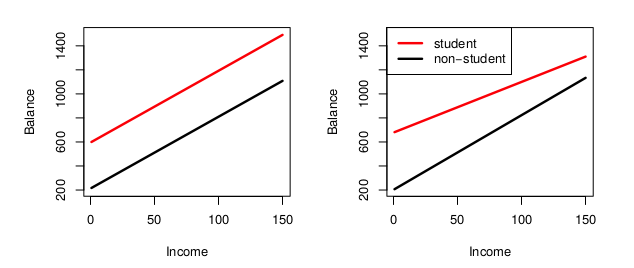
\includegraphics[width=1.\linewidth, height=0.5\textheight]{./img/graph01}
	\caption{IZQ: sin interacción ; DER: con interacción \cite{hastie02}}
\end{figure}
\end{frame}


\subsection{Overfitting}
\begin{frame}
	\frametitle{Modelo Lineal y Overfitting}
	\framesubtitle{Regularización}
	\begin{itemize}
		\item{¿Qué hacemos con el overfitting?}
		\item{Una forma es hacer \emph{model selection}...}
		\item{Otra es utilizar técnicas de regularización.}
		\item{El objetivo es introducir una restricción en la función de costo ($RSS$ - la función que se minimiza) y con eso forzar a los $\beta$} a reducir su valor \\
		\item{\textbf{Ridge:} 
			\begin{equation}
			CF = \sum_{i=1}^N(y_{i}-\beta_{0}\sum_{j=1}^p\beta_{j}x_{ij})^2 + \lambda\beta_{j}^2 = RSS + \lambda\beta_{j}^2
			\end{equation}}	
		\item{\textbf{LASSO:} 
			\begin{equation}
			CF = \sum_{i=1}^N(y_{i}-\beta_{0}\sum_{j=1}^p\beta_{j}x_{ij})^2 + \lambda|\beta_{j}| = RSS + \lambda|\beta_{j}|
			\end{equation}}	
	\end{itemize}
\end{frame}

\begin{frame}
	\frametitle{Modelo Lineal y Overfitting}
	\framesubtitle{Regularización}
	\begin{itemize}
		\item{Se parte de la minimización de $RSS$ habitual + una restricción $\lambda|\sum_{j=1}^p\beta_{j}|$ que tiene el efecto de reducir los coeficientes $\beta_{j}$ estimados}
		\item{$\lambda$ es un hiperparámetro del modelo que controla el impacto de la penalización y se estima mediante \emph{cross validation}}
		\item{Ridge se inventó originalmente para lidiar con el problema de la multicolinealidad. Sesga los coeficientes para reducir la varianza}
		\item{Ambos ``encogen'' los coeficientes hacia cero. LASSO, además, hace que algunos sean iguales a cero}
		\item{LASSO, entonces, realiza \emph{model selection}}
		\item{Es una formalización de un proceso que muchas veces se hace artesanalmente}
	\end{itemize}
\end{frame}


\begin{frame}[allowframebreaks] %allow to expand references to multiple frames (slides)

	\frametitle{Referencias bibliográficas}
		\scriptsize{\bibliographystyle{acm}}
		\bibliography{../bib/biblio} %bibtex file name without .bib extensio	n
\end{frame}



\end{document}